\documentclass{beamer}

\usepackage{verbatim}
\usepackage{fancyvrb}
\usepackage{amsmath}
\usepackage{mathtools}
\usepackage{booktabs}
\usepackage{amssymb}
\usepackage{graphicx}
\usepackage{calc}
\usepackage{color}
\usepackage{multicol}
\usepackage{wrapfig}
\usepackage{natbib}
\usepackage[ruled,vlined,linesnumbered]{algorithm2e}
\usepackage{animate}
\usepackage{mathtools}
\usepackage{listings}

\usepackage{cmbright}
\fontencoding{OT1}\fontfamily{cmbr}\selectfont %to load ot1cmbr.fd
\DeclareFontShape{OT1}{cmbr}{bx}{n}{% change bx definition
<->cmbrbx10%
}{}
\normalfont % back to normalfont

% two col: two columns
\newenvironment{twocol}[4]{
\begin{columns}[c]
\column{#1\textwidth}
#3
\column{#2\textwidth}
#4
\end{columns}
}

\makeatletter
\setbeamertemplate{theorem begin}
{%
\begin{\inserttheoremblockenv}
  {}{\usebeamerfont*{block title}\usebeamercolor[fg]{block title}%
  \inserttheoremname
  %\inserttheoremnumber
  \ifx \inserttheoremaddition \empty \else\ (\inserttheoremaddition)\fi
  \inserttheorempunctuation}
  \normalfont
  }
  \setbeamertemplate{theorem end}{\end{\inserttheoremblockenv}}
\makeatother

\newcommand{\E}{\mathrm{E}}
\newcommand{\Var}{\mathrm{Var}}
\newcommand{\Cov}{\mathrm{Cov}}
\newcommand{\sd}{\mathrm{sd}}
\newcommand{\s}{\mathrm{s}}
\newcommand{\Corr}{\mathrm{Corr}}
\newcommand{\rank}{\mathrm{rank}}
\newcommand{\trace}{\mathrm{trace}}
\newcommand{\nullspace}{\mathrm{null}}
\newcommand{\myspan}{\mathrm{span}}
\DeclareMathOperator*{\argmax}{arg\,max}
\DeclareMathOperator*{\argmin}{arg\,min}
\DeclareMathOperator*{\softmax}{softmax}
\DeclareMathOperator{\diag}{diag}

\definecolor{darkgreen}{rgb}{0,0.5,0}

\newtheorem{proposition}[theorem]{Proposition}
\newtheorem{exe}{Exercise}
\newtheorem{notation}{Notation}
\newtheorem{remark}{Remark}

\definecolor{darkgreen}{rgb}{0,0.5,0}

\title{Remedial Measures}
\author{Zhenisbek Assylbekov}
\institute{Department of Mathematics}
\date{Regression Analysis}

\AtBeginSection[]
{
  \begin{frame}<beamer>
    \tableofcontents[currentsection]
  \end{frame}
}

\begin{document}

\begin{frame}
  \titlepage
\end{frame}

\section{Weighted Least Squares}
\begin{frame}{Non-homogeneous variance}
\begin{columns}
\begin{column}{.4\textwidth}
\begin{figure}
    \centering
    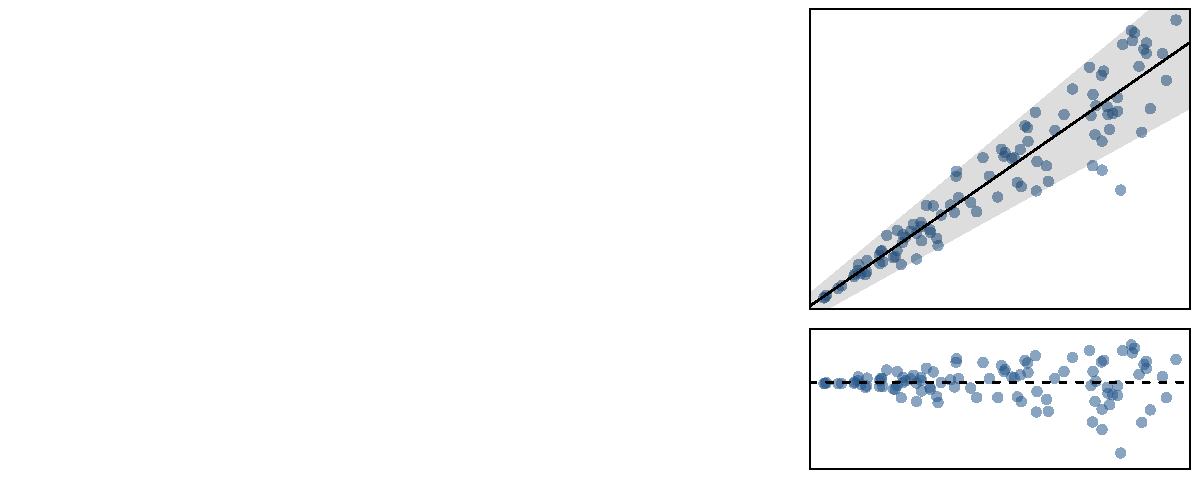
\includegraphics[width=.9\textwidth]{plots/heteroscedastic.pdf}
\end{figure}
\end{column}
\begin{column}{.6\textwidth}
\begin{itemize}
    \item Chapters 3 and 6 discuss transformations of $x_1, \ldots, x_k$ and/or $Y$.
    \item<2-> More advanced remedy: \textbf{weighted least squares} (WLS) regression.
    \item<3-> Model is as before
    $$
    Y_i = \beta_00 + \beta_1\cdot x_{i1} + \ldots + \beta_k\cdot x_{ik} + \epsilon_i,
    $$
    \item<4-> Except that
    $$
    \epsilon_i\,\,{\stackrel{\text{ind}}{\sim}}\,\,\mathcal{N}(0,\sigma^2_i)    
    $$
\end{itemize}
\end{column}
\end{columns}
\end{frame}

\begin{frame}{Weighted least squares}
\begin{itemize}
\item We have $\Var[Y_i] = \sigma_i^2$. 
\item<2-> Idea: Give observations with higher variance less
weight in the regression fitting.
\item<3-> Let $\omega_i=\frac{1}{\sigma^2_i}$. WLS solves
$$
\min_{\boldsymbol\beta}\sum_{i=1}^n\omega_i[Y_i-(\beta_0+\beta_1 x_{i1}+\ldots+\beta_k x_{ik})]^2
$$
\item<4-> Or in matrix notation:
$$\min_{\boldsymbol\beta}(\mathbf{Y}-\mathbf{X}\boldsymbol\beta)^\top\mathbf{\Omega}(\mathbf{Y}-\mathbf{X}\boldsymbol\beta)$$
where $\mathbf{\Omega}=\diag[\omega_1,\ldots,\omega_n]\in\mathbb{R}^{n\times n}$.
\end{itemize}
\end{frame}

\begin{frame}{Solving WLS}
    Let us rewrite the WLS objective as:
    \begin{align*}
        \hat{\boldsymbol{\beta}}_{\text{WLS}}&=\argmin_{\boldsymbol{\beta}}(\mathbf{Y}-\mathbf{X}\boldsymbol\beta)^\top\mathbf{\Omega}(\mathbf{Y}-\mathbf{X}\boldsymbol\beta)\\
        \onslide<2->{&=\argmin_{\boldsymbol{\beta}}(\mathbf{Y}-\mathbf{X}\boldsymbol\beta)^\top\mathbf{\Omega}^{1/2}\mathbf{\Omega}^{1/2}(\mathbf{Y}-\mathbf{X}\boldsymbol\beta)\\}
        \onslide<3->{&=\argmin_{\boldsymbol{\beta}}(\mathbf{\Omega}^{1/2}\mathbf{Y}-\mathbf{\Omega}^{1/2}\mathbf{X}\boldsymbol\beta)^\top(\mathbf{\Omega}^{1/2}\mathbf{Y}-\mathbf{\Omega}^{1/2}\mathbf{X}\boldsymbol\beta)\\}
        \onslide<4->{&=\argmin_{\boldsymbol{\beta}}\|\mathbf{\Omega}^{1/2}\mathbf{Y}-\mathbf{\Omega}^{1/2}\mathbf{X}\boldsymbol\beta\|^2\qquad\text{(This is OLS!)}}
    \end{align*}
    \onslide<5->{Hence}
    \begin{multline*}
    \onslide<5->{\hat{\boldsymbol\beta}_\text{WLS}=\left((\mathbf{\Omega}^{1/2}\mathbf{X})^\top(\mathbf{\Omega}^{1/2}\mathbf{X})\right)^{-1}\left(\mathbf{\Omega}^{1/2}\mathbf{X}\right)^\top\mathbf{\Omega}^{1/2}\mathbf{Y}}\\\onslide<6->{=(\mathbf{X}^\top\mathbf{\Omega}\mathbf{X})^{-1}\mathbf{X}^\top\mathbf{\Omega}\mathbf{Y}}
    \end{multline*}
\end{frame}

\begin{frame}{But $\sigma_i$'s are unknown!}
\begin{itemize}
    \item However, $\sigma_1,\ldots,\sigma_n$ are usually unknown!
    \item<2-> Notice, that in OLS 
    $$
    \E[e_i^2] = \Var[e_i]+(\E[e_i])^2=\Var[Y_i-\hat{Y}_i]=\sigma^2(1-h_{ii})
    $$
    \item<3-> So $e_i^2$ in OLS estimates $\sigma^2$
and $|e_i|$ estimates $\sigma$ if $h_{ii} \approx 0$.
    \item<4-> Look at plots of $|e_i|$ from an OLS fit against $x_i$'s and $\hat{Y}_i$'s to see how $\sigma$ changes with predictors or fitted values.
    \item<5-> For example, if $|ei|$ increases linearly with $\hat{Y}_i$, then we'll
    fit 
    $$
    |e_i| = \alpha_0 + \alpha_1\cdot x_{i1} + \ldots + \alpha_k\cdot x_{ik} + \delta_i
    $$ 
    and obtain the fitted values $\widehat{|e_i|}$.
    \item<6-> Or, e.g., if $|\epsilon_i|$ increases linearly w.r.t. $x_{i4}$ only, then we'll fit $|e_i|=\alpha_0+\alpha_1\cdot x_{i4}+\delta_i$
\end{itemize}
\end{frame}

\begin{frame}[fragile]{Putting it all together}
\begin{enumerate}
    \item Regress $Y$ against predictor variable(s) as usual (OLS), and obtain $e_1,\ldots, e_n$ \& $\hat{Y}_1, \ldots, \hat{Y}_n$.
    \item<2-> Regress $|e_i|$ against (all or some) predictors $x_1, \ldots, x_k$ or fitted values $\hat{Y}$.
    \item<3-> Let $\widehat{|e_i|}$ be the fitted values for the regression in 2.
    \item<4-> Define $\omega_i = 1/\widehat{|e_i|}^2$ and feed them into \verb|lm| command using the \verb|weights| parameter.
\end{enumerate}    
\end{frame}

\begin{frame}{Example: diastolic blood pressure vs age}
We are interested in studying the relationship between diastolic blood pressure and age among healthy adult women 20 to 60 years old.\\~\\

\pause Fitting an OLS $\text{dbp}_i=\beta_0+\beta_1\cdot\text{age}_i+\epsilon_i$ gives:
\begin{figure}
    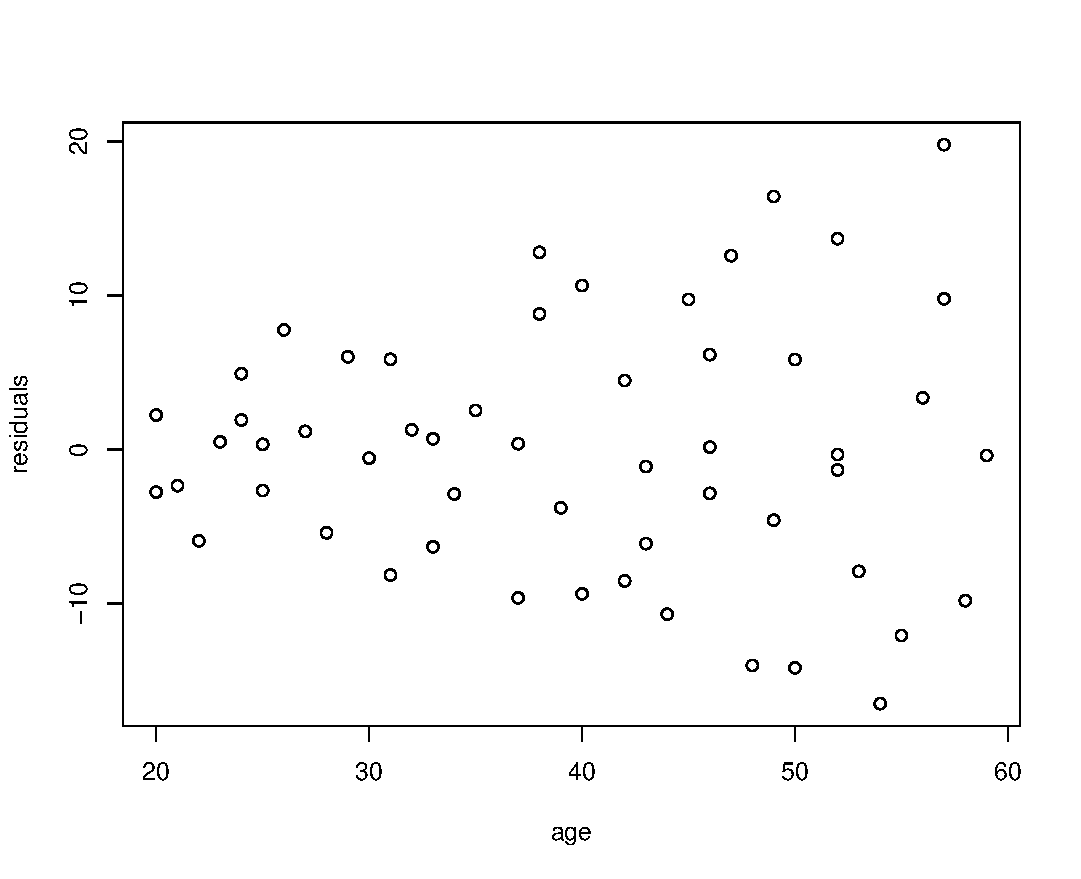
\includegraphics[width=.49\textwidth]{plots/res_age.pdf}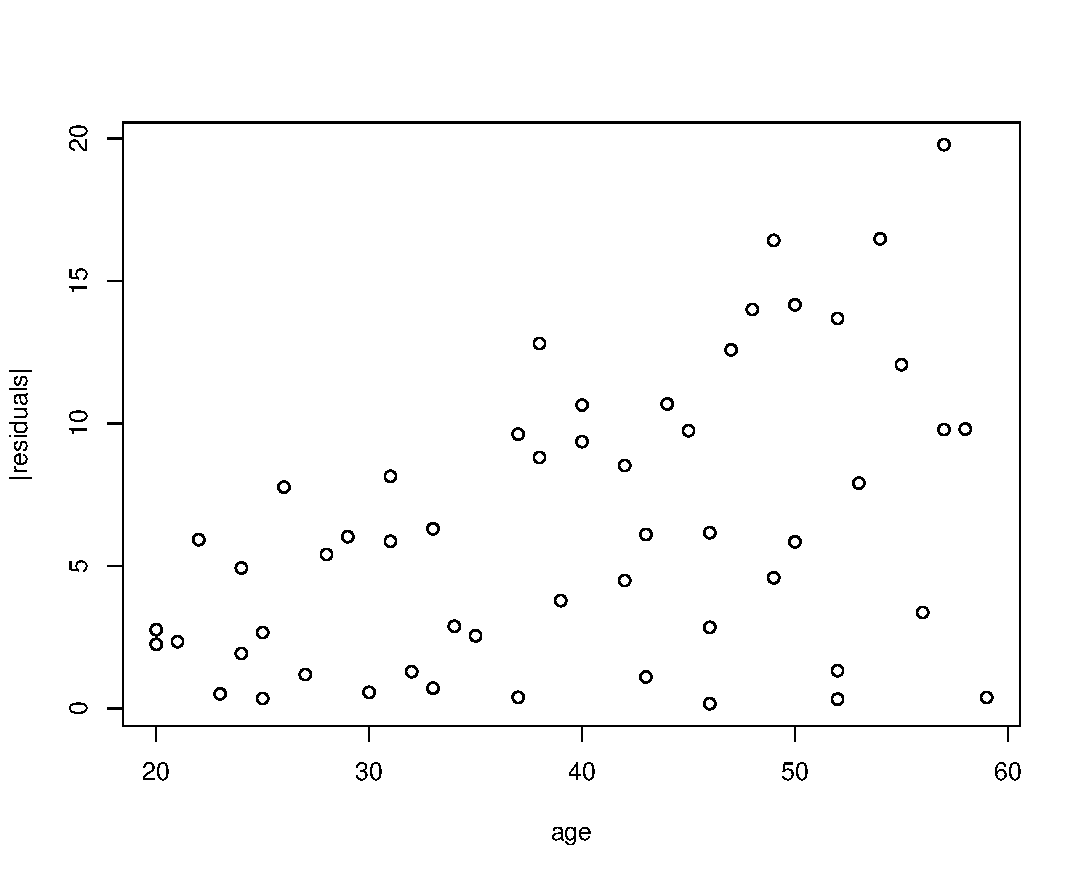
\includegraphics[width=.49\textwidth]{plots/abs_res_age.pdf}
\end{figure}    
\end{frame}

\begin{frame}[fragile]{OLS vs WLS}{\url{https://github.com/zh3nis/MATH440/blob/main/chp11/dbp.R}}
\begin{footnotesize}
\begin{verbatim}
> summary(ols)

Coefficients:
            Estimate Std. Error t value Pr(>|t|)    
(Intercept) 56.15693    3.99367  14.061  < 2e-16 ***
age          0.58003    0.09695   5.983 2.05e-07 ***
---
Residual standard error: 8.146 on 52 degrees of freedom
Multiple R-squared:  0.4077,	Adjusted R-squared:  0.3963 
\end{verbatim}
\pause\begin{verbatim}
> summary(wls)

Coefficients:
            Estimate Std. Error t value Pr(>|t|)    
(Intercept) 55.56577    2.52092  22.042  < 2e-16 ***
age          0.59634    0.07924   7.526 7.19e-10 ***
---
Residual standard error: 1.213 on 52 degrees of freedom
Multiple R-squared:  0.5214,	Adjusted R-squared:  0.5122 
\end{verbatim}
\end{footnotesize}
\end{frame}

\begin{frame}{Comments}
\begin{itemize}
    \item $\s[b_1]$ reduced from 0.097 (OLS) to 0.079 (WLS)
    \item<2-> $R^2$ is no longer interpreted the same way in terms of amount of total variability explained by model.
    \item<3-> In WLS, standard inferences about coefficients may not be valid for small sample sizes when weights are estimated from the data.
    \item<4-> If MSE of the WLS regression is near 1, then our estimation of the $\sigma_i$ function is okay. Here it's 1.21. 
\end{itemize}
\end{frame}


\section{Ridge Regression}
\begin{frame}{Ridge Regression}
If some predictors are collinear, then columns of $\mathbf{X}$ become linearly dependent, and $\mathbf{X}$ loses its rank.\\~\\
\onslide<2->{\structure{Exercise}: Show that for $\mathbf{X}\in\mathbb{R}^{n\times d}$ with $n\ge d$
$$
\mathrm{rank}(\mathbf{X})<d\quad\Rightarrow\quad\nexists\,{(\mathbf{X}^\top\mathbf{X})^{-1}}.
$$}%
\onslide<3->{This is bad for OLS, because $\mathbf{X}^\top \mathbf{X}$ will not be invertible.\\~\\

Simple solution: add penalty term into the cost function:
$$
Q(\boldsymbol{\beta})=\|\mathbf{Y}-\mathbf{X}\boldsymbol\beta\|^2+\lambda\|\boldsymbol{\beta}\|^2,
$$
where $\lambda$ is a \textit{hyperparameter}, to be chosen through a criterion like PRESS or training/validation approach.}
\end{frame}

\begin{frame}{Solving Ridge Regression}
\begin{theorem} The function $Q(\boldsymbol{\beta})=\|\mathbf{Y}-\mathbf{X}\boldsymbol\beta\|^2+\lambda\|\boldsymbol{\beta}\|^2$
reaches its minimum at
$$
\hat{\boldsymbol{\beta}}_{\text{R}}=(\mathbf{X}^\top\mathbf{X}+\lambda\mathbf{I})^{-1}\mathbf{X}^\top\mathbf{Y}
$$%
\end{theorem}
\begin{proof}
\vspace{-15pt}
\begin{align*}
\onslide<2->{Q(\boldsymbol\beta)&=}\onslide<3->{(\mathbf{Y}-\mathbf{X}\boldsymbol\beta)^\top(\mathbf{Y}-\mathbf{X}\boldsymbol\beta)+\lambda\boldsymbol\beta^\top\boldsymbol\beta\\}
\onslide<4->{&=\mathbf{Y}^\top\mathbf{Y}-\boldsymbol\beta^\top\mathbf{X}^\top\mathbf{Y}-\mathbf{Y}^\top\mathbf{X}\boldsymbol\beta+\boldsymbol\beta^\top\mathbf{X}^\top\mathbf{X}\boldsymbol\beta+\lambda\boldsymbol\beta^\top\mathbf{I}\boldsymbol\beta\\}
\onslide<5->{\nabla_{\boldsymbol\beta}Q&=-\mathbf{X}^\top\mathbf{Y}-\mathbf{X}^\top\mathbf{Y}+2\mathbf{X}^\top\mathbf{X}\boldsymbol\beta+2\lambda\mathbf{I}\boldsymbol\beta}\onslide<6->{\\&=2(\mathbf{X}^\top\mathbf{X}+\lambda\mathbf{I})\boldsymbol\beta-2\mathbf{X}^\top\mathbf{Y}}\onslide<7->{=\mathbf{0}\\}
\onslide<8->{&(\mathbf{X}^\top\mathbf{X}+\lambda\mathbf{I})\boldsymbol\beta=\mathbf{X}^\top\mathbf{Y}\quad\Rightarrow\quad}\onslide<9->{\boxed{\hat{\boldsymbol\beta}_\text{R}=(\mathbf{X}^\top\mathbf{X}+\lambda\mathbf{I})^{-1}\mathbf{X}^\top\mathbf{Y}}}
\end{align*}
\end{proof}

\onslide<10->{\structure{Exercise.} Show that $(\mathbf{X}^\top\mathbf{X}+\lambda\mathbf{I})$ is \textit{always} invertible for $\lambda>0$.}
\end{frame}

\begin{frame}{Chapter 7 example: Body fat}
$n=20$ healthy females 25--34 years old.
\begin{itemize}
\item $x_1=$ triceps skinfold thickness (mm)
\item $x_2=$ thigh circumference (cm)
\item $x_3=$ midarm circumference (cm)
\item $Y=$ body fat (\%)
\end{itemize}

Obtaining $Y_i$, the percent of the body that is purly fat, requires
immersing a person in water. Want to develop model based on simple body measurements that avoids people getting wet.
\end{frame}

\begin{frame}{Scatterplot}
\centering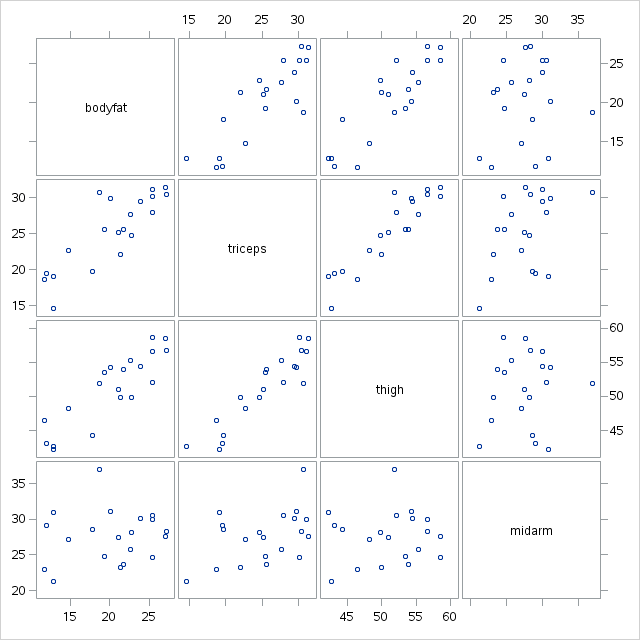
\includegraphics[scale=0.45]{plots/scatterplot}
\end{frame}

\begin{frame}{Correlation coefficients}
\begin{center}
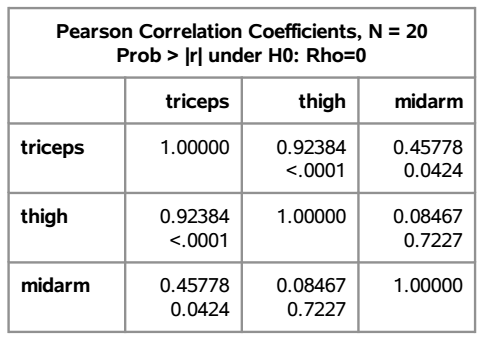
\includegraphics[scale=0.3]{plots/corr-matrix}
\end{center}
\pause There is high correlation among the predictors. \pause For example
$r = 0.92$ for triceps and thigh. These two variables are \textit{essentially
carrying the same information}. \pause Maybe only one or the other is really needed.
\end{frame}

\begin{frame}[fragile]{Effects of multicolinearity}
\begin{small}
\begin{verbatim}
lm(formula = bodyfat ~ triceps + thigh + midarm, 
   data = bodyfat_data)

Coefficients:
            Estimate Std. Error t value Pr(>|t|)
(Intercept)  117.085     99.782   1.173    0.258
triceps        4.334      3.016   1.437    0.170
thigh         -2.857      2.582  -1.106    0.285
midarm        -2.186      1.595  -1.370    0.190
\end{verbatim}
\end{small}

\begin{itemize}
    \item\pause Two of the three regression effects are {\it negative}.
    \item\pause Holding midarm
and triceps constant, increasing the thigh circumference {\it decreases} bodyfat.
    \item\pause This may not make sense!
\end{itemize}  
\end{frame}

\begin{frame}[fragile]{OLS vs Ridge on bodyfat data}{\url{https://github.com/zh3nis/MATH440/blob/main/chp11/ridge.R}}
\begin{columns}
\begin{column}{.6\textwidth}
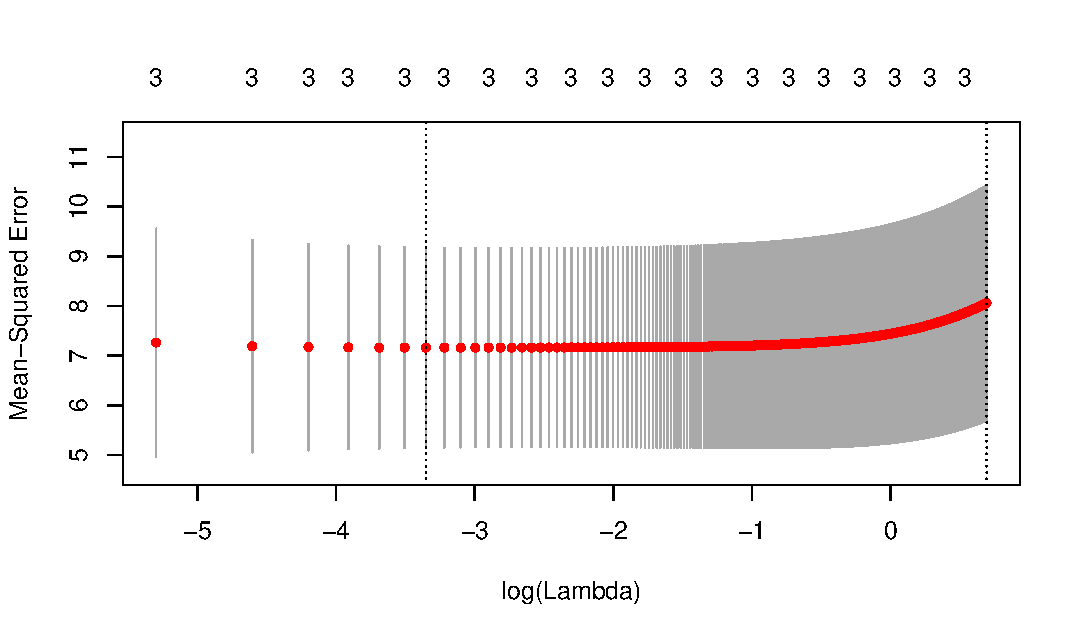
\includegraphics[height=.4\textheight]{plots/ridge_lambda.pdf}
\end{column}
\begin{column}{.4\textwidth}
\begin{footnotesize}
\begin{verbatim}
> mean(ols$residuals^2)
[1] 4.920244

> mean((y-ridge_yhat)^2)
[1] 5.340952
\end{verbatim}
\end{footnotesize}
\end{column}
\end{columns}
\begin{footnotesize}
\begin{verbatim}
> coef(ols)
(Intercept)     triceps       thigh      midarm 
 117.084695    4.334092   -2.856848   -2.186060 

> t(coef(ridge))
   (Intercept)   triceps     thigh     midarm
s0   0.6555753 0.8074414 0.1588796 -0.3266744
\end{verbatim}
\end{footnotesize}
\end{frame}

\section{Robust Regression}
\begin{frame}{Back to outliers}
\begin{itemize}
    \item Leverages $h_{ii}$ and deleted residuals $t_i$ useful for finding outlying $\mathbf{x}_i$ and $Y_i$ cases.
    \item\pause Cook's $D_i$ and $\text{DFFIT}_i$ indicate which cases are highly influencing the fit of the model.
    \item\pause What to do with influential and/or outlying cases? Are they transcription errors or somehow (un)representative of the target population?
    \item\pause Outliers are often interesting in their own right and can help in building a better model.
    \item\pause \textbf{Robust regression} weakens the effect of outlying cases on estimation to provide a better fit to the majority of cases.
    \item\pause Useful in situations when there's no time for ``influence diagnostics'' or a more careful analysis.
\end{itemize}
\end{frame}

\begin{frame}{M-estimation}
\begin{itemize}
    \item Robust regression is effective when the error distribution is not normal, but heavy-tailed.
    \item\pause \textbf{M-estimation} is a general class of estimation methods. \pause
    $$
    \min_{\boldsymbol\beta}\sum_{i=1}^n\rho(Y_i-\mathbf{x}_i^\top\boldsymbol\beta)
    $$
    \pause where $\rho(\cdot)$ is some function.
    \item\pause $\rho(u)=u^2$ gives OLS
    \item\pause $\rho(u)=|u|$ gives \textbf{least absolute residual} (LAR) regression
    \item\pause Huber's method is a compromise between OLS and LAR. \pause It looks like $u^2$ for $u$ around zero, and like $|u|$ for $u$ further away from zero.
\end{itemize}
\end{frame}

\begin{frame}{Iteratively reweighted least squares (IRLS)}
\begin{small}
Outlying residuals are (iteratively) given less weight in the estimation process.\\~\\

\begin{algorithm}[H]
\DontPrintSemicolon
\textbf{Input}: $\{(\mathbf{x}_i, {y}_i)\}_{i=1}^n$\;
Fit OLS. Let $\mathbf{e}=\mathbf{y}-\mathbf{X}\hat{\boldsymbol\beta}_\text{OLS}$\;
Initialize weights: $\omega_i\leftarrow\frac{1}{e_i^2}$, $\mathbf{\Omega}=\diag[\omega_1,\ldots,\omega_n]$\;
Fit WLS: $\hat{\boldsymbol\beta}_{\text{WLS}}\leftarrow(\mathbf{X}^\top\mathbf{\Omega X})^{-1}\mathbf{X}^\top\mathbf{\Omega}\mathbf{Y}$\;
Estimate: $\hat{\sigma}\leftarrow\mathrm{median}_i\left\{\frac{|y_i-\mathbf{x}_i^\top\hat{\boldsymbol\beta}_{\text{WLS}}|}{\Phi^{-1}(0.75)}\right\}$\;
Update weights: $\omega_i\leftarrow w\left(\frac{y_i-\mathbf{x}_i^\top\hat{\boldsymbol\beta}_{\text{WLS}}}{\hat{\sigma}}\right)$, where
$$
w(u)=\begin{cases}
1,\quad &|u|<1.345\\
\frac{1.345}{|u|},&|u|>1.345
\end{cases}
$$\;\vspace{-10pt}
Repeat steps 4--6 until $\hat{\sigma}$ and $\hat{\boldsymbol\beta}_{\text{WLS}}$ stabilize.\;
\textbf{Output}: $\hat{\boldsymbol\beta}_{\text{WLS}}$
\caption{IRLS}
\end{algorithm}
\end{small}
\end{frame}

\begin{frame}[fragile]{IRLS example}{\url{https://github.com/zh3nis/MATH440/blob/main/chp11/irls.R}}
\begin{verbatim}
require(foreign)
require(MASS)

cdata <- read.dta(
    "https://stats.idre.ucla.edu/stat/data/crime.dta")

plot(crime ~ poverty, data=cdata)
ols <- lm(crime ~ poverty, data = cdata)
abline(ols)

irls <- rlm(crime ~ poverty, data=cdata)
abline(irls, col='blue')

summary(ols)
summary(irls)
\end{verbatim}    
\end{frame}

\begin{frame}{IRLS example}
\begin{figure}
    \centering
    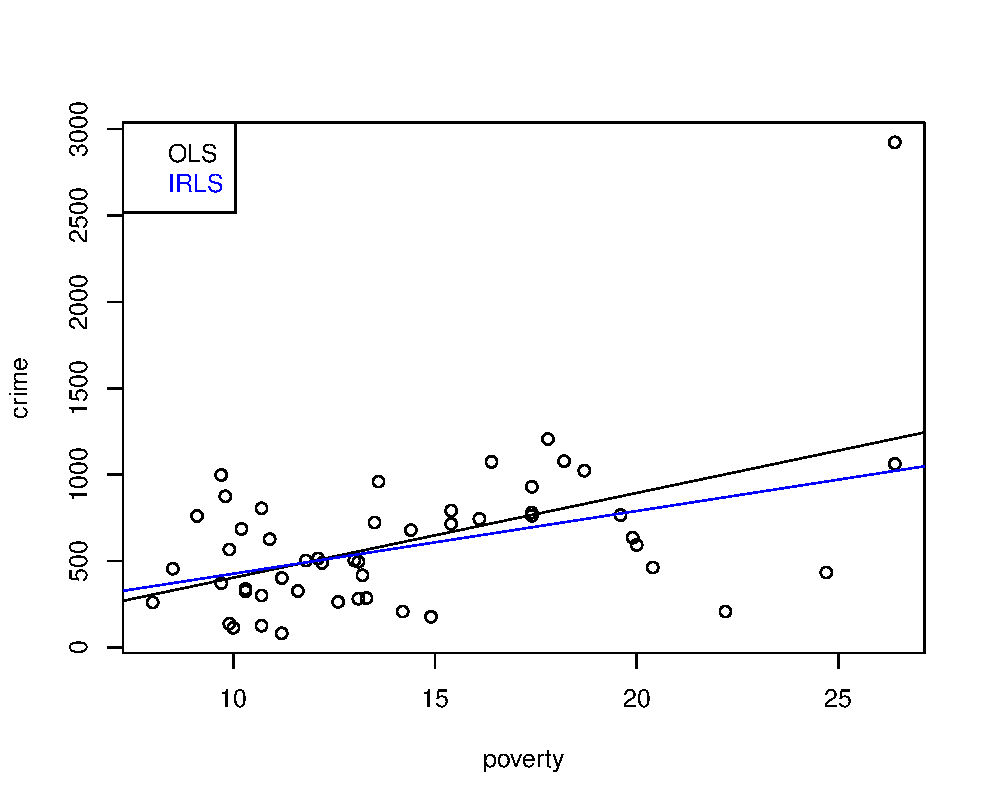
\includegraphics[width=.9\textwidth]{plots/ols_irls.pdf}
\end{figure}
\end{frame}

\end{document}